
\section{Wahrscheinlichkeiten}

% ------------------------------------------------------------------------------------------------ %
% Ereignissraum
% ------------------------------------------------------------------------------------------------ %

\subsection{Ereignisraum, Grundraum}

\begin{definition}[Ereignisraum]
	Der \emph{Ereignisraum} oder \emph{Grundraum} \(\Omega\) ist die Menge aller möglichen Ereignisse eines Zufallexperiments. Die Elemente \(\omega \in \Omega\) heissen \emph{Elementarereignisse}.
\end{definition}

\begin{definition}[Ereignis]
	Ein \emph{Ereignis} \(A \subseteq \Omega\) ist eine Teilmenge von \(\Omega\).
\end{definition}

Die Klasse aller \emph{beobachtbaren Ereignisse} \(\mathcal{F}\) ist eine Teilmenge der Potenzmenge \(\mathcal{P}(\Omega)\) von \(\Omega\).


% ------------------------------------------------------------------------------------------------ %
% Das Wahrscheinlichkeitsmass
% ------------------------------------------------------------------------------------------------ %


\subsection{Wahrscheinlichkeitsmass}

\begin{definition}[Wahrscheinlichkeitsmass]
	Ein \emph{Wahrscheinlichkeitsmass} \(\P\) ist eine Abbildung \(\P:\mathcal{F} \rightarrow [0,1]\) mit folgenden Eigenschaften:
	\begin{compactenum}[i:]
		\item \(\P[\Omega] = 1\).
		\item \(\P[A] \geq 0\) für alle \(A \in \mathcal{F}\).
		\item \(\P[\bigcup_{i=1}^\infty A_i] = \sum_{i=1}^\infty \P[A_i]\) falls \(A_i \cap A_j = \emptyset\) für \(i \neq j\).
	\end{compactenum}
\end{definition}

Aus den Axiomen i bis iii folgen direkt die Rechenregeln:
\begin{compactenum}[i:]
	\item \(\P[A^C] = 1 - \P[A]\).
	\item \(\P[\emptyset] = 0\).
	\item \(A \subseteq B \Rightarrow \P[A] \leq \P[B]\).
	\item \(\P[A \cup B] = \P[A]+\P[B]-\P[A \cap B]\) (\emph{Additionsregel}).
	\item \(\P[B] = \P[B \cap A] + \P[B \cap A^C]\)
\end{compactenum}

\begin{definition}[Endliche Räume]
	Für \emph{endliche Räume} \(\Omega = \{\omega_1,\ldots,\omega_n\}\) gilt:\\
	\(\P[A] = \sum_{ w_i \in A} \P[w_i]\)
\end{definition}

\begin{definition}[Laplace-Raum]
	Im \emph{Laplace-Raum} sind alle Ereignisse gleich wahrscheinlich:
	\(P[A] = \frac{\lvert A \rvert}{\lvert \Omega \rvert}\)
\end{definition}

% ------------------------------------------------------------------------------------------------ %
% BEDINGTE WAHRSCHEINLICHKEIT, TOTALE WAHRSCHEINLICHKEIT UND FORMEL VON BAYES
% ------------------------------------------------------------------------------------------------ %


\subsection{Bedingte Wahrscheinlichkeit}

\begin{definition}[Bedingte Wahrscheinlichkeit]
	Für Ereignisse \(A,B\) mit \(\P[A] > 0\) ist die \emph{bedingte Wahrscheinlichkeit} definiert durch:
	\[
		\P[B \mid A] := \frac{\P[A \cap B]}{\P[A]}
	\]
\end{definition}

Es folgt die \emph{Multiplikationsregel}:
\(\P[A \cap B] = \P[B \mid A] \P[A]\)

\begin{theorem}[Totale Wahrscheinlichkeit]
	Sei \(A_{1 \leq i \leq n}\) eine Partitionierung von \(\Omega\), dann gilt für ein beliebiges Ereignis \(B\):
	\[
		\P[B] = \sum_{i=1}^n \P[B \mid A_i]\P[A_i]
	\]
\end{theorem}

\begin{theorem}[Formel von Bayes]
	Sei \(A_1,\ldots,A_n\) eine Partitionierung von \(\Omega\) mit \(\P[A_i] > 0\) für alle \(i\) und \(B\) ein Ereignis mit \(\P[B] > 0\), dann gilt für jedes \(k\):
	\[
		\P[A_k \mid B] = \frac{\P[B \mid A_k] \P[A_k]}{\P[B]}
		= \frac{\P[B \mid A_k] \P[A_k]}{\sum_{i=1}^n \P[B \mid A_i] \P[A_i]}
	\]
\end{theorem}

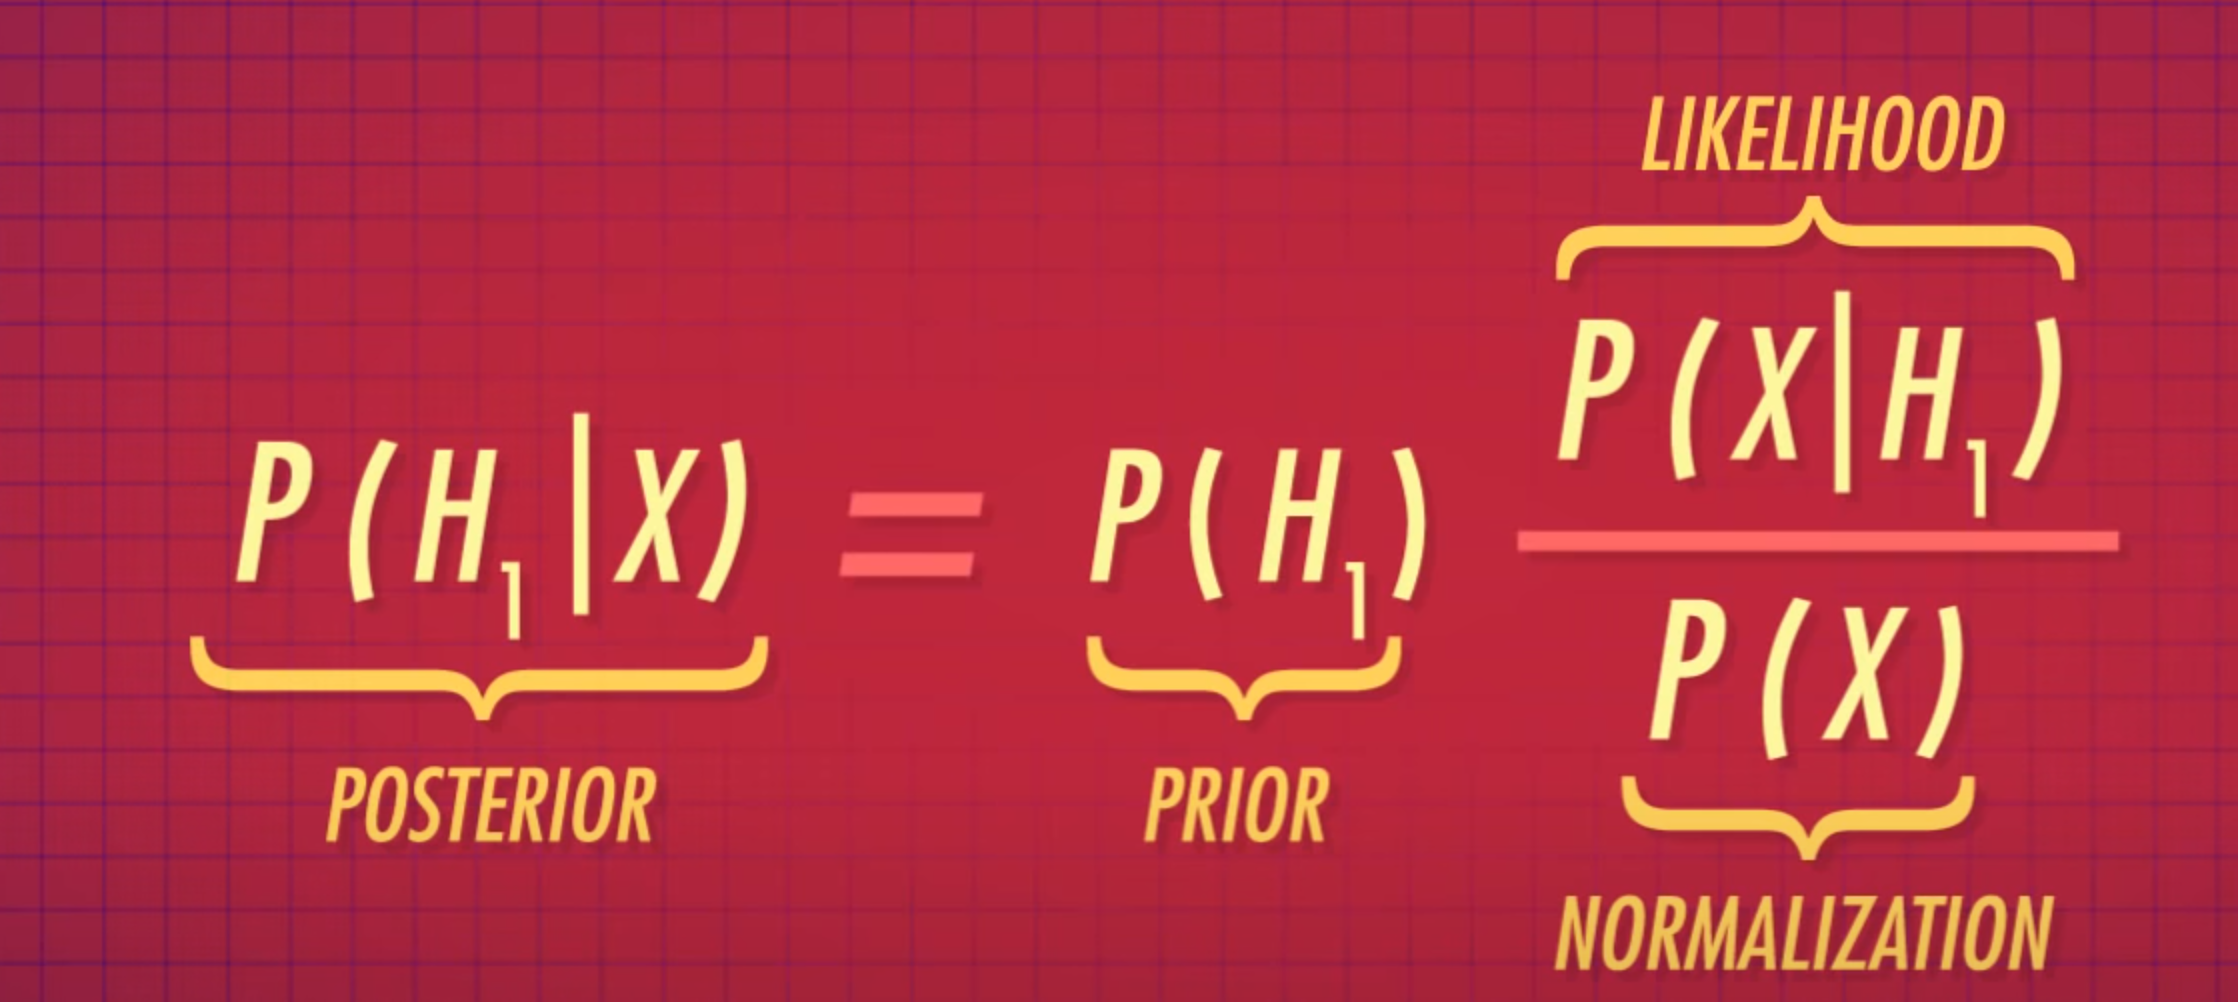
\includegraphics[width=.5\textwidth]{images/prior_posterior.png}

% ------------------------------------------------------------------------------------------------ %
% UNABHÄNGIGKEIT
% ------------------------------------------------------------------------------------------------ %

\begin{definition}[Unabhängigkeit]
	Zwei Ereignisse \(A,B\) heissen \emph{unabhängig} \(A \perp B\), wenn \(\P[B \mid A] = \P[B] \) gilt. \(\Rightarrow \P[A \cap B] = \P[A] \P[B]\)
\end{definition}
% ------------------------------------------------------------------------------------------------ %
